% Some classes load the `subfigure` package which clashes with
% our internal use of `subfig` for subfloats. We are most likely
% not going to need the canned subfigure functionality anyways,
% so we'll trick LaTeX into thinking it already loaded `subfigure`
\makeatletter
\newcommand{\dontusepackage}[2][]{%
  \@namedef{ver@#2.sty}{9999/12/31}%
  \@namedef{opt@#2.sty}{#1}}
\makeatother
\dontusepackage{subfigure}


%% ===== Begin LaTeX file ===========================
%%
\documentclass[]{pandoc/sigchi}

\usepackage{lmodern}
\usepackage{amssymb,amsmath}
\usepackage{ifxetex,ifluatex}
\usepackage[usenames,dvipsnames]{color}
\usepackage{fixltx2e} % provides \textsubscript
\ifnum 0\ifxetex 1\fi\ifluatex 1\fi=0 % if pdftex
  \usepackage[T1]{fontenc}
  \usepackage[utf8]{inputenc}
\else % if luatex or xelatex
  \ifxetex
    \usepackage{mathspec}
    \usepackage{xltxtra,xunicode}
  \else
    \usepackage{fontspec}
  \fi
  \defaultfontfeatures{Mapping=tex-text,Scale=MatchLowercase}
  \newcommand{\euro}{€}
\fi
% use upquote if available, for straight quotes in verbatim environments
\IfFileExists{upquote.sty}{\usepackage{upquote}}{}
% use microtype if available
\IfFileExists{microtype.sty}{%
\usepackage{microtype}
\UseMicrotypeSet[protrusion]{basicmath} % disable protrusion for tt fonts
}{}
% disbable natbib, sigchi template handles that by itself
%\usepackage[]{natbib}
\bibliographystyle{pandoc/SIGCHI-Reference-Format}
\usepackage{listings}
% Define slightly more reasonable Listings defaults
\lstset{
    basicstyle=\ttfamily\small,
    breaklines=true,
    prebreak=\raisebox{0ex}[0ex][0ex]{\ensuremath{\hookleftarrow}},
    frame=lines,
    showtabs=false,
    showspaces=false,
    showstringspaces=false,
    keywordstyle=\color[gray]{0.4}\bfseries,
    commentstyle=\color[gray]{0.65}\itshape,
    numbers=left,
    captionpos=b,
}
\ifxetex
  \usepackage[setpagesize=false, % page size defined by xetex
              unicode=false, % unicode breaks when used with xetex
              xetex]{hyperref}
\else
  \usepackage[unicode=true]{hyperref}
\fi
\hypersetup{breaklinks=true,
            bookmarks=true,
            pdfauthor={Maxime Daniel; Guillaume Rivière; Nadine Couture},
            pdftitle={Interfaces Tangibles comme Aide à la Maitrise de l'Énergie},
            colorlinks=true,
            citecolor=black,
            urlcolor=blue,
            linkcolor=black,
            pdfborder={0 0 0}}
\urlstyle{same}  % don't use monospace font for urls
\setlength{\parindent}{0pt}
\setlength{\parskip}{6pt plus 2pt minus 1pt}
\setlength{\emergencystretch}{3em}  % prevent overfull lines
\setcounter{secnumdepth}{-2}

%% from sigchi
% useful for balancing the last columns
\usepackage{balance}


\title{Interfaces Tangibles comme Aide à la Maitrise de l'Énergie}
\author{Maxime Daniel \and Guillaume Rivière \and Nadine Couture}
\date{}


% comment if you want LaTeX's default font
\usepackage{times}

% we'll override the "\caption*" that scholdoc uses with default figure markup
\usepackage{suffix}

% explicitely load subfig 'cause we won't use scholdoc touchy subfigures
\usepackage{subfig}


\begin{document}

% need a loop 'cause there is subfields
      \teaser{
      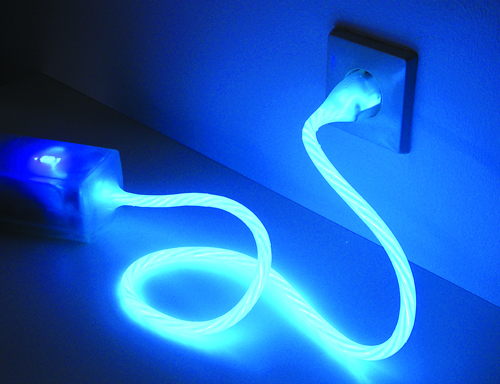
\includegraphics[width=\textwidth]{./images/powerawarecord.jpg}
      \caption{Power-Aware Cord\label{fig:teaser}}
    }
  
\maketitle
\begin{abstract}
TO DO.
\end{abstract}

\keywords{
      IHM;
      TUI;
      Technologie persuasive;
      Espace public et physique d'interaction sociale}

      \category{TO DO}{TO DO}{TO DO}
  

% from natbib commands to apalike + make it work in captions
\def \citep {\protect\cite}

%% From demo file

% Arabic page numbers for submission. 
% Remove this line to eliminate page numbers for the camera ready copy
\pagenumbering{arabic}

% llt: Define a global style for URLs, rather that the default one
\makeatletter
\def\url@leostyle{%
  \@ifundefined{selectfont}{\def\UrlFont{\sf}}{\def\UrlFont{\small\bf\ttfamily}}}
\makeatother
\urlstyle{leo}

% To make various LaTeX processors do the right thing with page size.
\def\pprw{8.5in}
\def\pprh{11in}
\special{papersize=\pprw,\pprh}
\setlength{\paperwidth}{\pprw}
\setlength{\paperheight}{\pprh}
\setlength{\pdfpagewidth}{\pprw}
\setlength{\pdfpageheight}{\pprh}

% Make sure hyperref comes last of your loaded packages, to give it a
% fighting chance of not being over-written, since its job is to
% redefine many LaTeX commands.
\definecolor{linkColor}{RGB}{6,125,233}
\hypersetup{%
  bookmarksnumbered,
  colorlinks,
  citecolor=black,
  filecolor=black,
  linkcolor=black,
  urlcolor=linkColor,
  breaklinks=true,
}

% we'll override the "\caption*" that scholdoc uses with default figure markup
\WithSuffix\newcommand\caption*{\caption}% *-variant

% In case we got a problem with scholdoc headers' levels
% from http://tex.stackexchange.com/a/61803
\newcommand{\leveldown}% Demote sectional commands
  {\let\section\subsection%
   \let\subsection\subsubsection%
   \let\subsubsection\paragraph%
   \let\paragraph\subparagraph%
   %\let\subparagraph\relax%
  }
  
\newcommand{\levelup}% Promote sectional commands
  {\let\subparagraph\paragraph%
   \let\paragraph\subsubsection%
   \let\subsubsection\subsection%
   \let\subsection\section%
   %\let\section\relax%
  }

% auto margin with subfigures
% FIXME: slight shift toward right...
\let\oldsubfloat\subfloat
\renewcommand*{\subfloat}{\hfill\oldsubfloat}


% promote all sections
\levelup

\chapter{Contexte}\label{contexte}

\chapter{Problématique}\label{probluxe9matique}

\chapter{Etat de l'art}\label{etat-de-lart}

\chapter{Technologie persuasive}\label{technologie-persuasive}

En 2002, Fogg introduit la persuasion à l'informatique avec ses travaux
sur les technologies persuasives \citep{fogg2002persuasive}. Il définis
les technologies persuasives comme des systèmes interactifs concus pour
le changer les attitudes et/ou les comportements et la persuasion comme
une tentative de redefinition, de renforcement, ou de changement de
comportements, de sentiments ou de pensées.

\chapter{Technologie persuasive
ambiante}\label{technologie-persuasive-ambiante}

\subsection{Définir la persuasion}\label{duxe9finir-la-persuasion}

La persuasion formule, renforce, ou change les comportements,
sentiments, ou pensées à propos d'un problème, d'un objet, ou d'une
action. \citep{fogg2002persuasive}

% to put before content of last page
\balance{}

\renewcommand\refname{Références}
\bibliography{resources/biblio}


\end{document}

